\section{Hubble's Law and SN Ia Cosmology}

\subsection{What the heck is a rest frame?}

Let's say you have some data, but it's from a supernova with $z = 0.1$. Because of the relativistic Doppler effect, the wavelengths you \textit{observe} are different from the ``actual'' wavelengths, i.e., rest frame wavelengths. It's called \textit{red}shift for a reason---observed wavelengths will be longer, or redder, than the rest frame wavelengths. This effect will also affect observed flux. Your observed flux is smaller than your rest frame flux because longer wavelengths are less energetic than shorter ones. Ignoring ejecta velocity (see Section \ref{sec:ejectavelocity}), this is why a spectral line won't appear in its ``expected'', or rest frame, position. Usually, you want to put your spectra in the rest frame before doing anything with them because it's hard to compare SNe at different redshifts. See Section~\ref{sec:spec_restframe} for details on correcting SN spectra to the rest frame. 

\subsection{$z_{helio}$ and $z_{CMB}$}

You'll encounter two kinds of redshift---heliocentric redshift ($z_{helio}$) and CMB (Cosmic Microwave Background) redshift ($z_{CMB}$). \textit{These are different, and are used for different purposes!} $z_{CMB}$ is the redshift caused by the Universe's expansion \textit{only}, i.e., where the reference frame is the CMB frame. $z_{helio}$ is the redshift with \textit{only} the Earth's rotation and orbit removed. There are still effects from other motion, like Galactic rotation and the Galaxy moving around with respect to other objects, as well as $z_{CMB}$. ``Heliocentric'' $\equiv$ ``Sun at center'', so ``Sun at center'' is the rest frame. It's how things are moving relative to the Milky Way. Note that $z_{helio}$, while often reported as an object's redshift, is \textit{not} the observed redshfit. The observed redshift does not have the Earth's rotation and orbit removed. In other words, $z_{helio}$ contains information about a bunch of things moving relative to each other, including motion relative to the CMB, while $z_{CMB}$ contains information about \textit{only} motion relative to the CMB.

For cosmology, you'll use $z_{CMB}$ (e.e., when making a Hubble diagram or determining other cosmological parameters). If you're dealing with data that you need to correct to the rest frame, you probably want to use $z_{helio}$.

\subsection{Peculiar velocity and the Hubble flow}
\label{sec:vpec}
If you're reading this section, you may have heard the term ``smooth Hubble flow'' thrown around a few times. But what \textit{is} this thing?

for one, not all of the components of a galaxy's velocity are moving away in accordance with the Universe's expansion. This is called the \textit{Hubble flow}---if an object is \textit{only} moving due to expansion (mostly), then it's in the Hubble flow. Any velocity deviation from the Hubble flow is called \textit{peculiar velocity}. For example, if a galaxy is under gravitational influence from another galaxy, the components of its motion due to that interaction is part of its peculiar velocity. However, this is hard to quantify, so it's usually assumed that peculiar velocity is around 300 km/s. You'll notice that in plots that show peculiar velocity error, like in the lower panel of Figure \ref{fig:hresid}, the error due to peculiar velocity gets smaller as an object is farther away. 

Peculiar velocity error is calculated as:
\begin{equation}
\label{eqn:evpec}
    \sigma_{v_{pec}} = \Big( \frac{5}{\ln 10} \Big) \Big( \frac{v_{pec}}{cz} \Big)
\end{equation}
So, it's a function of $z$! This makes sense---the farther away something is, the faster it's moving in the Hubble flow, so the peculiar velocity is a relatively small portion of its net velocity vector. 

\subsection{How to make a Hubble diagram}
Firstly, what is a Hubble diagram? It's a plot of recession velocity ($y$-axis) vs. distance ($x$-axis) (Figure \ref{fig:oghubble}). Turns out these things are positively correlated. In plain English, the farther away a galaxy is, the faster it's hurtling away from us (and everything else---the Universe is homogeneous and isotropic). This means the Universe is expanding\footnote{It's expanding at an accelerating rate, but this statement and a very crude Hubble diagram alone do not imply accelerated expansion}!

\begin{figure}[h!]
    \centering
    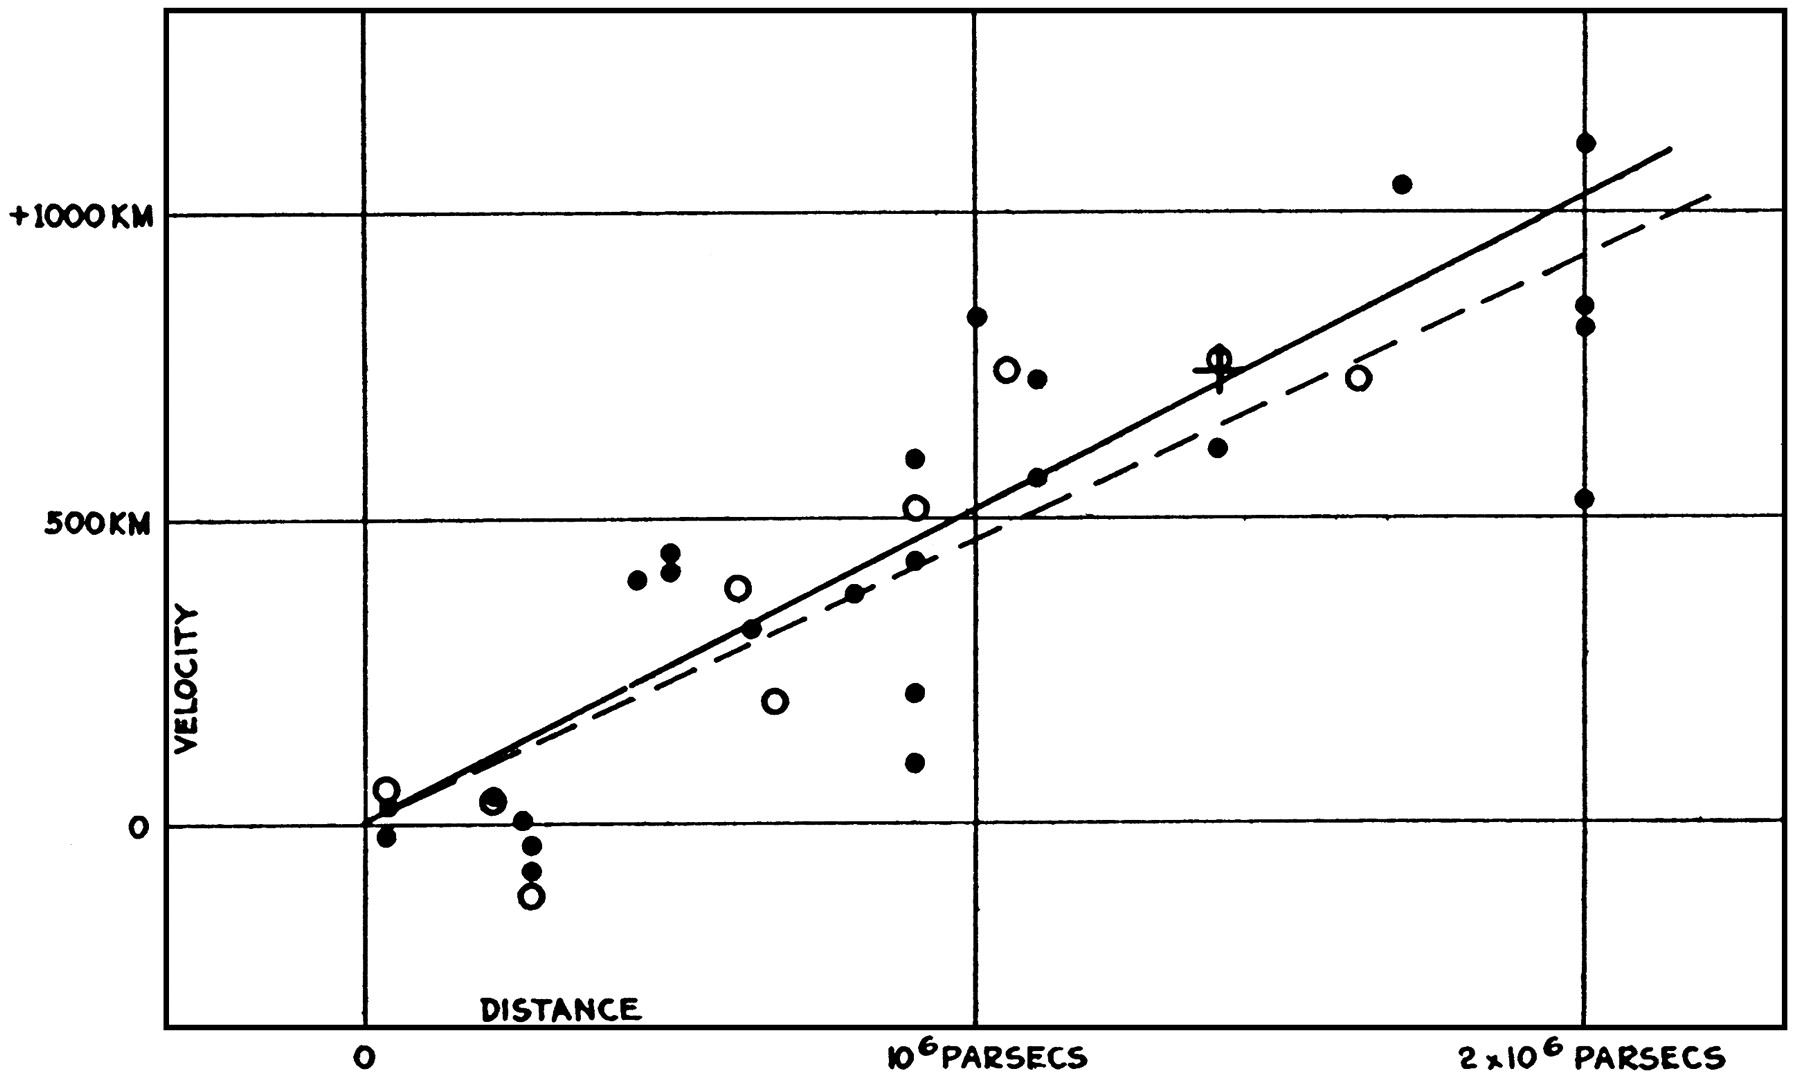
\includegraphics[width=0.7\textwidth]{figs/hubble_diagram_og.jpeg}
    \caption{The OG Hubble diagram. Note that the velocity units are km---\textit{this is a mistake}. It should probably be km/s. Even Edwin Hubble made an error on his most famous published figure. You're doing just fine.}
    \label{fig:oghubble}
\end{figure}

However, no one really uses linear distance units, like parsecs, or velocities like parsecs per second in Hubble diagrams in the literature any more. You still might see these, though. Units you may see to represent recession velocity on the $y$-axis include:
\begin{itemize}
    \item km/s
    \item The distance modulus $\mu$ (apparent magnitude minus absolute magnitude, $m-M$.)
\end{itemize}
Units you may see to represent distance on the $x$-axis include:
\begin{itemize}
    \item Mpc
    \item $z$
    \item log($z$) or log($cz$)
\end{itemize}
You'll most commonly see the distance modulus. It's the difference between apparent magnitude, $m$, and absolute magnitude, $M$. So, if the difference between these quantities is large, then an object is further away. If the difference is small, it's closer. You can think of $M$ as the intrinsic brightness of an object. $m$ is the brightness that you observe, corrected for effects like dust extinction (and because we're supernova people, also stuff like the luminosity-decline rate relation). 

So, there are many ways you can actually make a Hubble diagram because there are a zillion ways to standardize SNe Ia. I'll discuss $\chi^{2}$ minimization i Section~\ref{sec:chisq}. 

\subsection{Hubble residual}
The Hubble residual is the difference between the observed distance modulus of an SN and the expected distance modulus, obtained by fitting a cosmology to the data. This is important because this quantifies the uncertainty in our cosmological parameters. So, a lot of work is centered around minimizing the Hubble residual. 

\begin{figure}[h!]
    \centering
    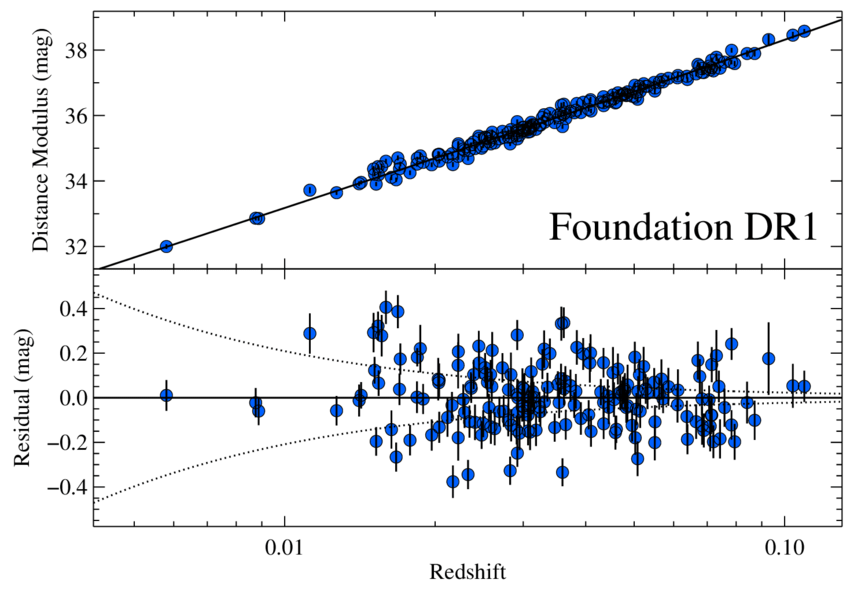
\includegraphics[width=0.8\textwidth]{figs/hubble-resid.png}
    \caption{A Hubble diagram (top) made with SNe Ia. The Hubble residual is plotted in the lower panel. The curved dotted lines in the lower panel mark error due to peculiar velocity. Figure from \cite{Foley2017}.}
    \label{fig:hresid}
\end{figure}

The curved dotted lines in Figure~\ref{fig:hresid} are estimated error due to peculiar velocity (Section~\ref{sec:vpec}, Equation~\ref{eqn:evpec}), usually assumed to be around 300 km s$^{-1}$. While you'll plot those curved dotted lines as peculiar velocity error alone, you should add the error due to peculiar velocity in quadrature (i.e. sum the errors like $\sigma = \sqrt{a^{2} + b^{2}}$) to the error bars on your data.

It's important to correct your $z$ for peculiar velocity---it influences your results \cite{Peterson2022}! You can get your peculiar velocity values using \href{https://github.com/laldoroty/pvhub/tree/make_installable}{this Python package, called \texttt{pvhub}}. The code is originally written by Erik Peterson for \cite{Peterson2022}. This paper has a really good overview of the different components of $z$, so check it out. For the purposes of this section, we care about correcting $z_{CMB}$ for $v_{pec}$. So, I'll parrot what's in that paper for a sentence or two. We go from $v_{pec}$ to $z_{pec}$ like this:
\begin{equation}
    z_{pec} = \frac{v_{pec}}{c},
\end{equation}

and correct $z_{CMB}$ like this:

\begin{equation}
\label{eqn:vpeccorrection}
    z_{cosmo} = \frac{1 + z_{CMB}}{1 + z_{pec}} - 1.
\end{equation}

\subsubsection{Troubleshooting}
\textbf{My Hubble residual shows a slight trend}: this could be becuase you need to correct $z_{CMB}$ for the effects of peculiar velocity. See Equation~\ref{eqn:vpeccorrection}.\\

\noindent\textbf{My scatter is just... enormous}: if you used least squares minimization, check that (1) you typed your $\chi^{2}$ expression correctly, and (2) that you're inputting the correct arrays (e.g., if you accidentally put in $m_{B}$ where $\sigma_{m_{B}}$ should be). 

\subsection{Important papers for supernova cosmology}

\textit{The Use of Supernovae Light Curves for Testing the Expansion Hypothesis and Other Cosmological Relations}, B. Rust's PhD thesis, 1974 \cite{Rust1974}. The author shows that SNe Ia can be used to test the expanding Universe hypothesis.\\

\noindent\textit{Light curves, color curves, and expansion velocity of type I supernovae as functions of the rate of brightness decline}, I. Pskovskii 1977 \cite{Pskovskii1977}. This is the first paper to quantify the rate of brightness decline. It was quantified as $\beta$, which paved the way for $\Delta m_{15}$ much later \cite{Phillips1993}. \\

\noindent\textit{The Absolute Magnitudes of Type Ia Supernovae}, M. Phillips 1993 \cite{Phillips1993}. This paper shows that the absolute magnitudes of SNe Ia are correlated with the decline rate of the $B-$band light curve. This paper is why the luminosity-decline relation is sometimes called the ``Phillips relation''. This paper quantifies the brightness decline rate as $\Delta m_{15}$---the change in magnitude from the date of maximum brightness to 15 days later.\\

\noindent\textit{Dr. Paulina Lira's Masters thesis}, 1995. This thesis notes a linear region in the color curve (color vs. time) of SNe Ia. This is suggested as a method to correct reddening. \\

\noindent\textit{The Reddening-Free Decline Rate Versus Luminosity Relationship for Type IA Supernovae}, M. Phillips et al. 1999. \cite{Phillips1999}. This paper elaborates on Phillips 1993 \cite{Phillips1993}. It modifies the previously-described luminosity-decline relation by correcting for host galaxy extinction using the relation in Lira 1995.\\

\noindent\textit{Observational Evidence from Supernovae for an Accelerating Universe and a Cosmological Constant}, Riess et al. 1998 \cite{Riess1998}. This is the paper that won the Nobel Prize in 2011, awarded to Adam Riess, Saul Perlmutter, and Brian Schmidt. The authors used High-$z$ Supernova Search Team data combined with some nearby SNe to show that the distances of the high $z$ SNe were larger than expected, implying that the Universe is expanding at an accelerating rate. The Supernova Cosmology Project group found the same results at around the same time.\\